\section{Présentation et caractéristiques des machines}\label{sec:contribs:machines}

Nous présentons dans cette section deux machines NUMA de générations et de caractéristiques différentes.
La première, \emph{idchire}, est basée sur des processeurs Intel Sandy Bridge, et possède un nombre important de nœuds NUMA.
La seconde, \emph{brunch}, est basée sur des processeurs Intel plus récents de la génération Broadwell, et dispose d'un nombre assez faible de nœuds NUMA.

\subsection{idchire}\label{sec:contribs:machines:idchire}

La machine idchire a été fabriquée par SGI, modèle UV 2000~\cite{uv2000}.
Elle est équipée de 24 processeurs Intel(R) Xeon(R) CPU E5-4640 (Sandy Bridge), cadencés à 2.4 GHz.
Chacun de ces processeurs est associé à 31 Go de RAM pour former un nœud NUMA, et dispose de 8 cœurs physiques partageant 20 Mo de cache L3 (20-ways associatif).
Chacun des cœurs a accès à 32 Ko de cache L1 (données) et 256 Ko de cache L2 (8-ways associatif).
Les latences et bandes passantes relatives à chacun des niveaux de cache sont présentées dans le tableau~\ref{tab:synthese-processeurs}.

La machine entière dispose donc de 192 cœurs physiques, et de 744 Go de RAM.
Les processeurs Sandy Bridge disposent de l'extension vectorielle AVX, permettant d'effectuer 4 additions et 4 multiplications de nombres flottant à double précision en un cycle, portant le pic de performance théorique de la machine à 3.6 TFLOPs.

\subsubsection{Topologie}

\begin{figure}[ht]
  \centering
  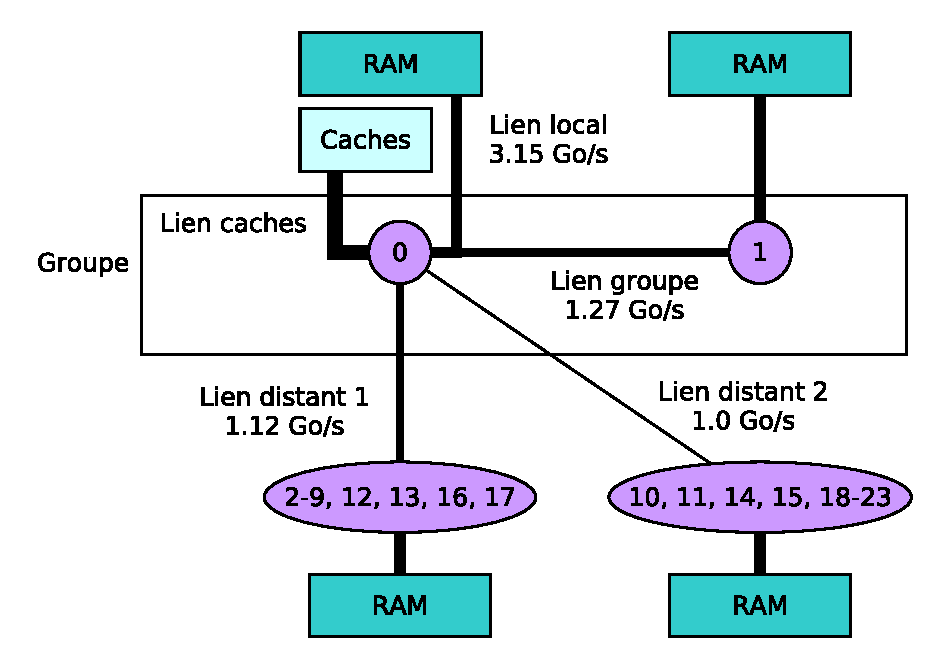
\includegraphics[width=0.8\textwidth]{topo-idchire}
  \caption{Topologie schématique vu du nœud 0}\label{fig:contribs:machines:idchire:topo-liens}
\end{figure}

L'interconnexion des nœuds NUMA est effectué à travers l'Intel \emph{Quick Path Interconnect} (QPI).
La topologie de la machine expose une hiérarchie à plusieurs niveaux, la Figure~\ref{fig:contribs:machines:idchire:topo-liens} présente la hiérarchie de la machine du point de vue du nœud 0.
Chaque nœud est d'abord associé à un autre nœud pour former un groupe. Ces groupes sont ensuite interconnectés entre eux et sont accessibles en deux rebonds maximum dans le système d'interconnexion.
Pour chaque nœud il y a 12 nœuds situés à un rebond, et 10 nœuds situés à deux rebonds.

\begin{figure}[t!]
  \centering
  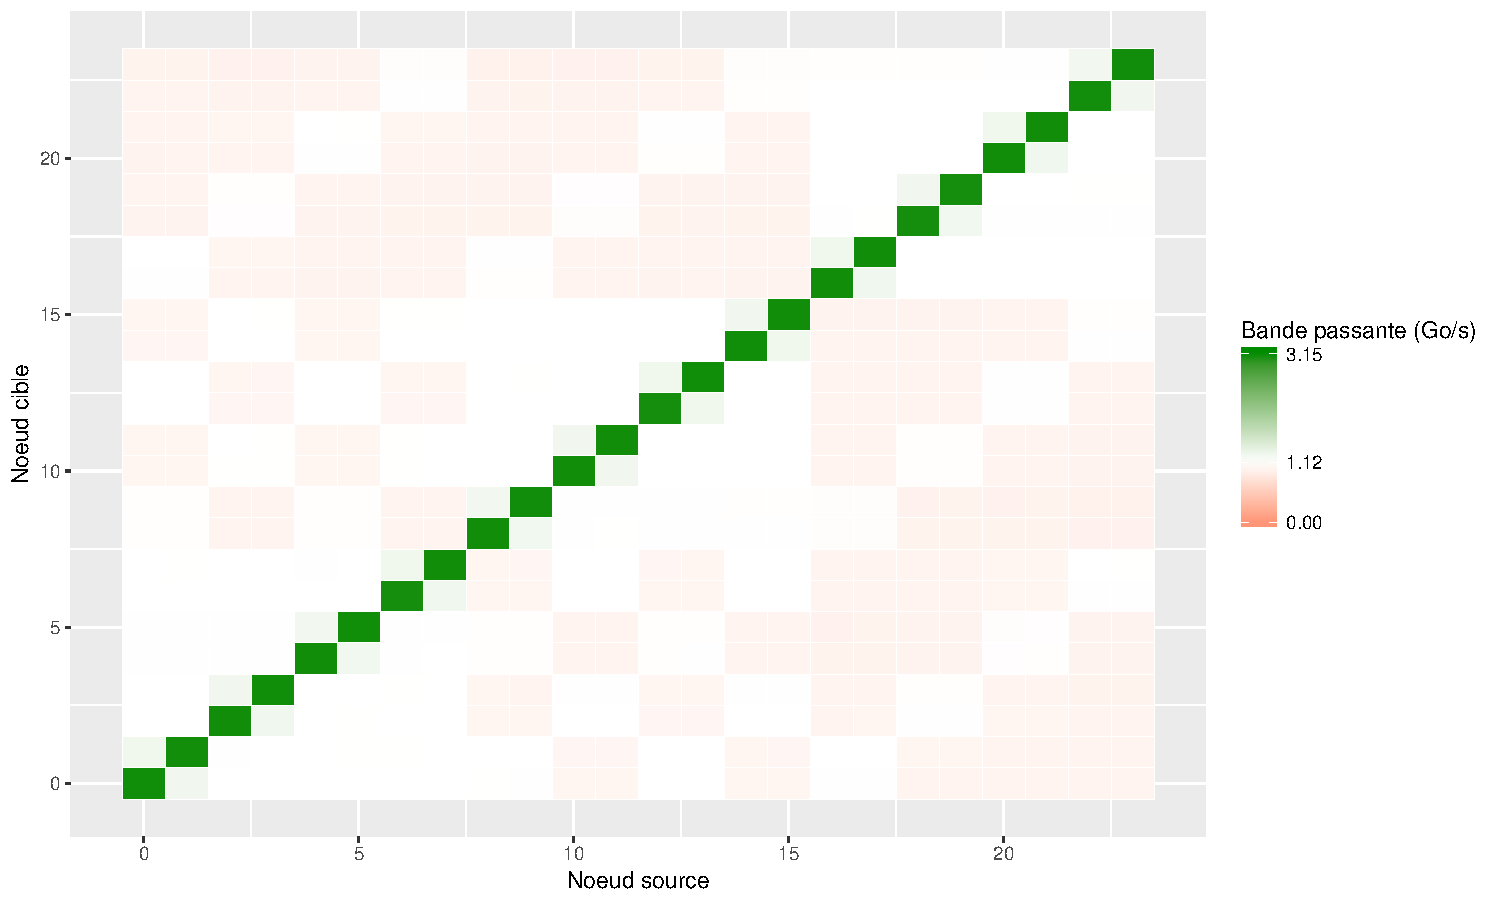
\includegraphics[width=\textwidth]{heatmap_idchire_memcpy}
  \caption{Carte de la bande passante d'idchire}\label{fig:contribs:machines:idchire:heatmap}
\end{figure}

\begin{figure}[h!]
  \centering
  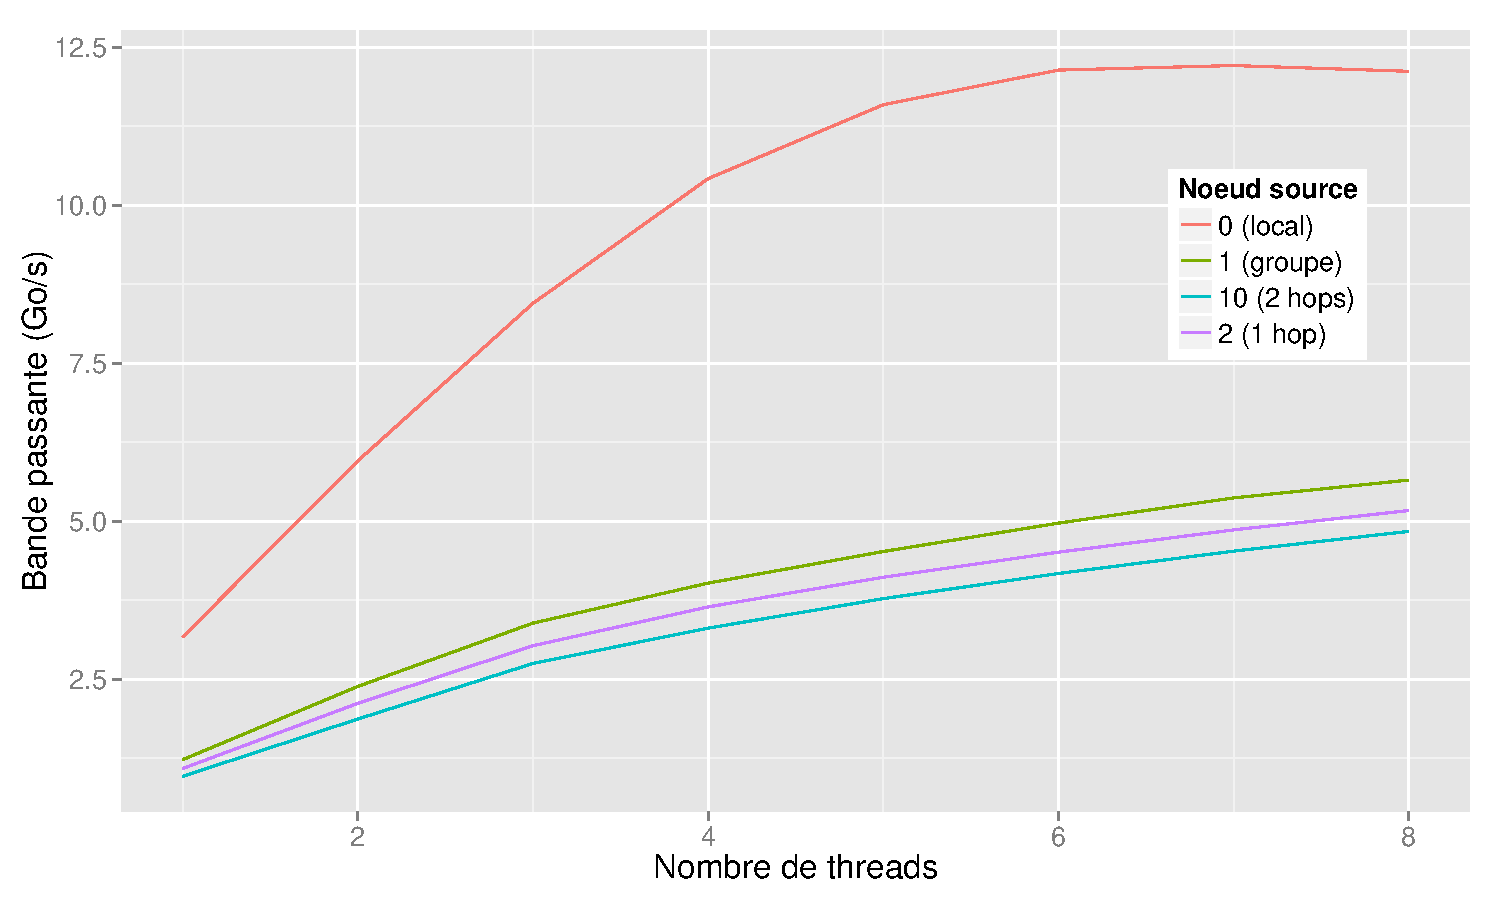
\includegraphics[width=0.9\textwidth]{link_saturation}
  \caption{Bande passante cumulée vers le nœud 0, en fonction du nombre de threads effectuant une copie et du nœud source}\label{fig:contribs:machines:idchire:saturation}
\end{figure}


La Figure~\ref{fig:contribs:machines:idchire:heatmap} présente la bande passante nœud à nœud, en fonction du nœud source et du nœud destination.
La mesure est via une copie de tableau (|memcpy|) de 200 Mo, entre un tableau alloué et initialisé sur le nœud source, et un tableau alloué sur le nœud destination.
Elle fait apparaître clairement une diagonale où la bande passante est significativement plus grande, illustrant le coût d'un accès mémoire local comparé à un accès distant.
On peut également constater que la bande passante point à point est symétrique.

Vu du nœud 0 et en point à point, on a donc 4 niveaux de bande passante en fonction du lien utilisé~: 3.15 Go/s pour le lien local, 1.27 Go/s pour le lien du groupe, 1.12 Go/s pour le lien distant avec 1 hop, et enfin 1.0 Go/s pour le lien distant avec 2 hops.

Ces mesures permettent de quantifier la pénalité d'un accès distant, mais la simple <<carte>> obtenue ne suffit pas à caractériser complètement les temps d'accès aux nœuds NUMA, puisque qu'une seule communication ne va pas saturer la bande passante totale disponible, ni même illustrer l'impact de la contention.


\subsubsection{Mesure des liens}\label{sec:contribs:machines:idchire:liens}

En dehors de l'accès aux caches locaux, il y a 4 liens à quantifier, identifiés sur la Figure~\ref{fig:contribs:machines:idchire:topo-liens}.
Afin de mesurer la largeur de chacun des liens, nous avons défini des scénarios spécifiques pour mesurer la bande passante en entrée du nœud 0, en fonction du nœud distant possédant la donnée.

Le scénario est le suivant~: deux tableaux de 200 Mo sont alloués, un sur le nœud 0, et un qui est alloué et initialisé sur un autre nœud, qui est le nœud source.
La seule action est une copie du tableau distant (via |memcpy|), depuis le nœud source vers le nœud 0, et exécutée sur un cœur du nœud 0.

Étant donné qu'il y a 8 cœurs sur le nœud 0, nous avons effectué jusqu'à 8 copies simultanées (effectuées sur des tableaux indépendants).

L'annexe~\ref{chap:annexe:tool:bp} donne l'exemple du scénario utilisé pour la saturation du lien <<groupe>>, qui effectue de 1 à 8 copie simultanées depuis le nœud 1 vers le nœud 0, et qui a permis de générer la courbe verte dans la figure~\ref{fig:contribs:machines:idchire:saturation} (nœud source 1).

La figure~\ref{fig:contribs:machines:idchire:saturation} regroupe les résultats de la bande passante cumulée, en fonction du nombre de copies simultanées ayant lieu, et en fonction du nœud d'où provient les données.
Faire les copies depuis le nœud 0 permet de quantifier la largeur du lien local (qui atteint au maximum 12.2 Go/S)~;
les copies depuis le nœud 1 permettent de quantifier le lien groupe (qui plafonne à 5.6 Go/s)~;
les copies depuis le nœud 2 permettent de quantifier le lien distant avec 1 hop (au maximum 5.1 Go/s)~;
et enfin les copies depuis le nœud 10 permettent de quantifier le lien distant avec 2 hops, qui atteint au maximum 4.8 Go/s.

\begin{figure}[ht]
  \centering
  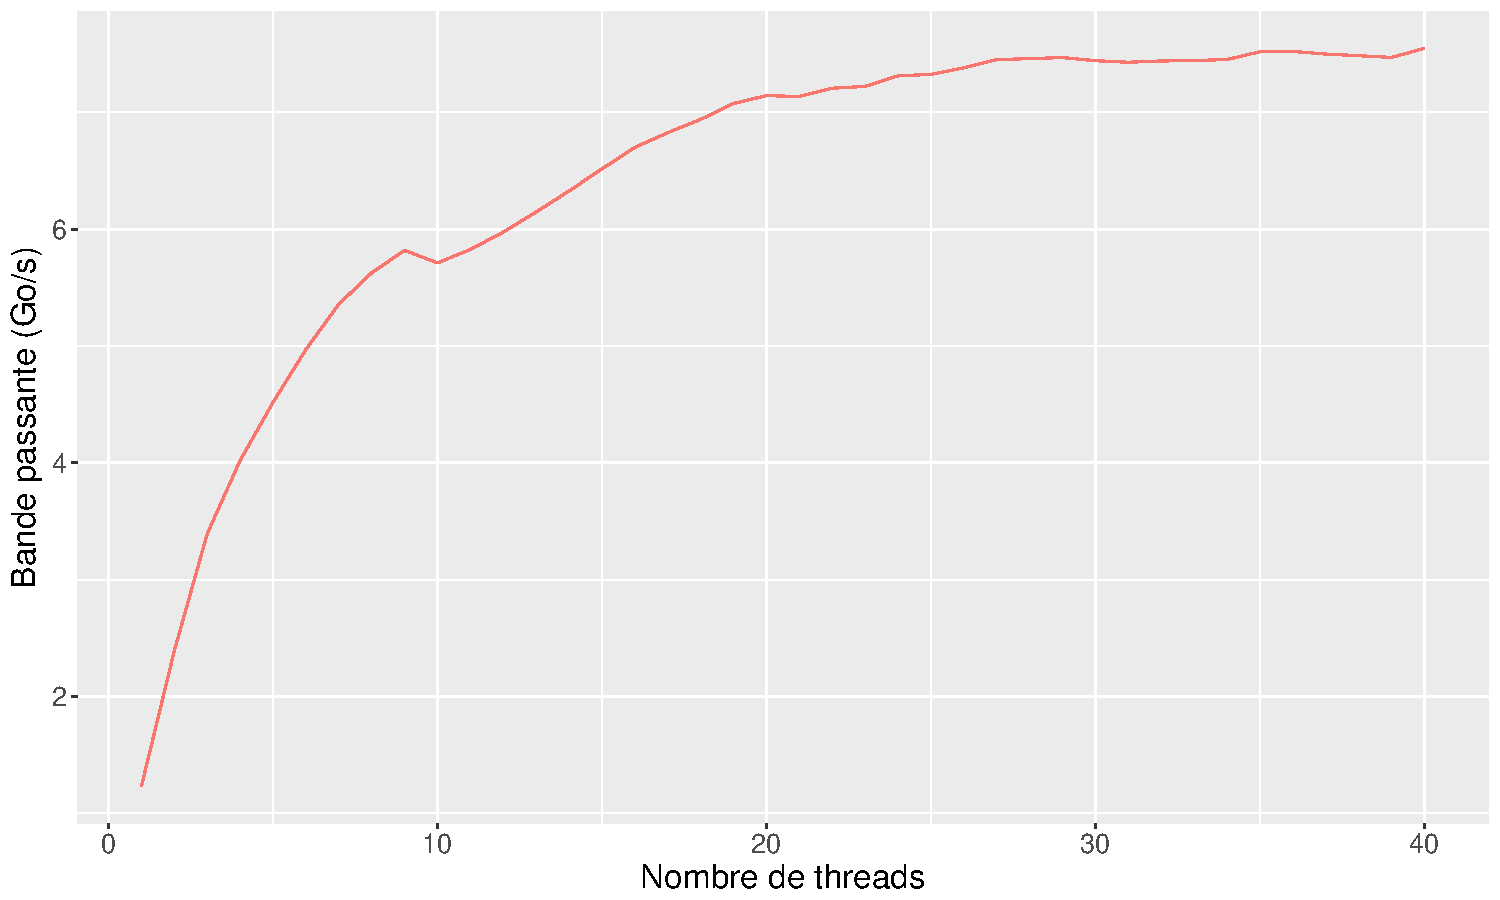
\includegraphics[width=0.9\textwidth]{link_output_saturation}
  \caption{Bande passante cumulée depuis le nœud 0 vers plusieurs nœuds distants, en fonction du nombre de threads distants effectuant une copie}\label{fig:contribs:machines:idchire:saturation-output}
\end{figure}

Pour terminer la caractérisation de ces liens, nous avons finalement mesuré la bande passante maximale que l'on peut obtenir en <<sortie>> d'un nœud, en saturant les différents liens.
Pour ce faire nous allons effectuer simultanément plusieurs copies d'un tableau de 200 Mo alloué et initialisé sur le nœud 0, vers un tableau alloué sur un nœud distant. Le thread effectuant la copie est placé sur le nœud distant.

La figure~\ref{fig:contribs:machines:idchire:saturation-output} montre la bande passante cumulée lors d'une copie du nœud 0 vers plusieurs nœuds distants, en fonction du nombre de threads effectuant une copie.
Pour cette expérience la manière de placer les threads sur les nœuds distants est importante~: les threads sont d'abord placés de manière à remplir progressivement le nœud 1 (nombre de threads de 1 à 8), qui passent par le lien groupe~; puis ce sont les nœuds 2, 3, et 4 qui sont remplis progressivement (threads 9 à 32), qui passent par le lien distant 1, et enfin le nœud 10 est rempli (threads 33 à 40), qui passent par le lien distant 2.

La bande passante maximale en sortie de nœud est donc de 7.5 Go/s, et commence à saturer aux alentours d'une vingtaine de copies distantes.


\subsection{brunch}\label{sec:contribs:machines:brunch}

Cette machine est équipée de 4 processeurs Intel(R) Xeon(R) CPU E7-8890 v4 (Broadwell), cadencés à 2.2 GHz.

Chacun de ces processeurs est associé à 378 Go de RAM pour former un nœud NUMA, ils disposent de 24 cœurs physiques partageant 60 Mo de cache L3 (20-ways associatifs).
Chacun des cœurs a accès à 32 Ko de cache L1 (données) et 256 Ko de cache L2.
Les latences et bandes passantes relatives à chacun des niveaux de cache sont présentées dans le tableau~\ref{tab:synthese-processeurs}.

La machine entière dispose donc de 96 cœurs physiques, et de 1.5 To de RAM.
Les processeurs Broadwell disposent d'instructions FMA~\footnote{\emph{Fused Multiply-Add}, permettant d'effectuer une addition et une multiplication en une étape}, permettant d'effectuer 8 additions et multiplications de nombres flottants à double précision en un cycle, portant le pic de performance théorique de la machine à 3.3 TFLOPs.


\subsubsection{Topologie}

\begin{figure}[ht]
  \centering
  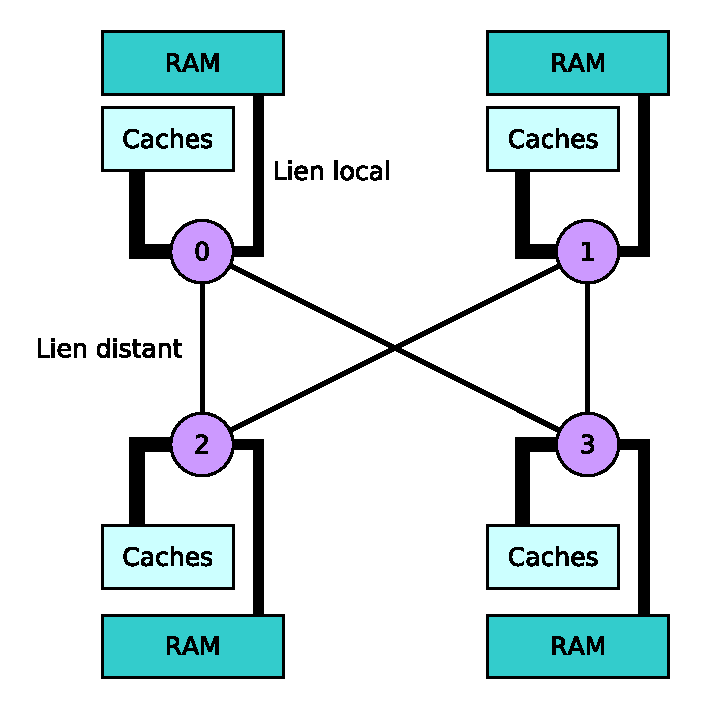
\includegraphics[width=0.6\textwidth]{topo-brunch}
  \caption{Topologie schématique complète de brunch}\label{fig:contribs:machines:brunch:topo-liens}
\end{figure}

L'interconnexion des nœuds NUMA est effectuée à travers l'Intel \emph{Quick Path Interconnect} (QPI).
Contrairement à idchire, la topologie de la machine est relativement plate~: les nœuds sont directement connectés les uns aux autres, et seule la notion d'accès distant ou local permet de distinguer une hiérarchie.
La topologie complète de la machine est représentée sur la figure~\ref{fig:contribs:machines:brunch:topo-liens}

\begin{figure}[t!]
  \centering
  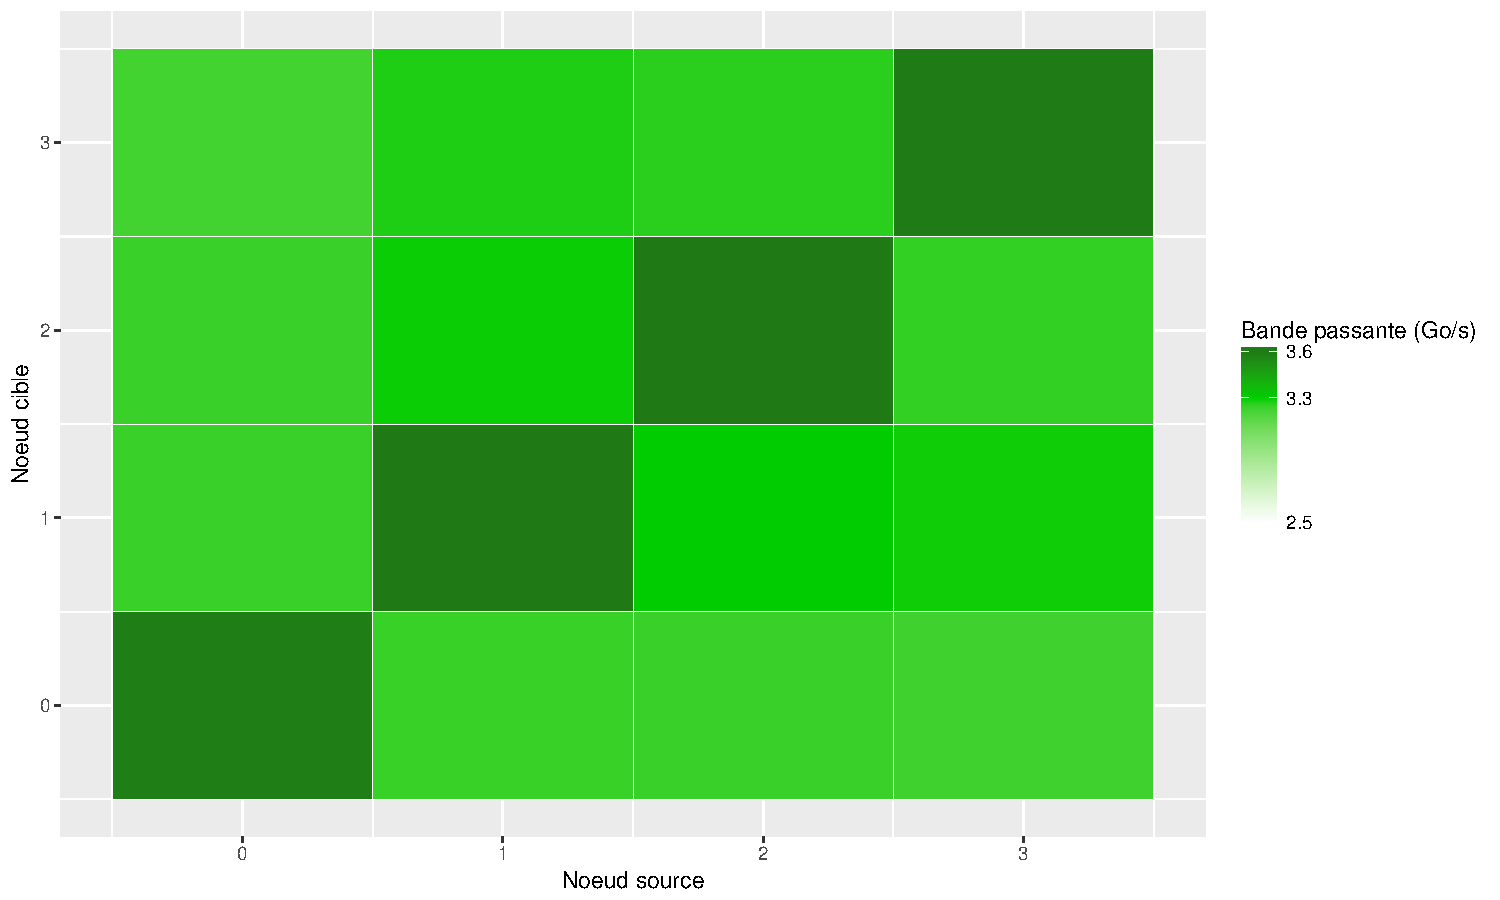
\includegraphics[width=\textwidth]{heatmap_brunch}
  \caption{Carte de la bande passante de brunch}\label{fig:contribs:machines:brunch:heatmap}
\end{figure}
\begin{figure}[h!]
  \centering
  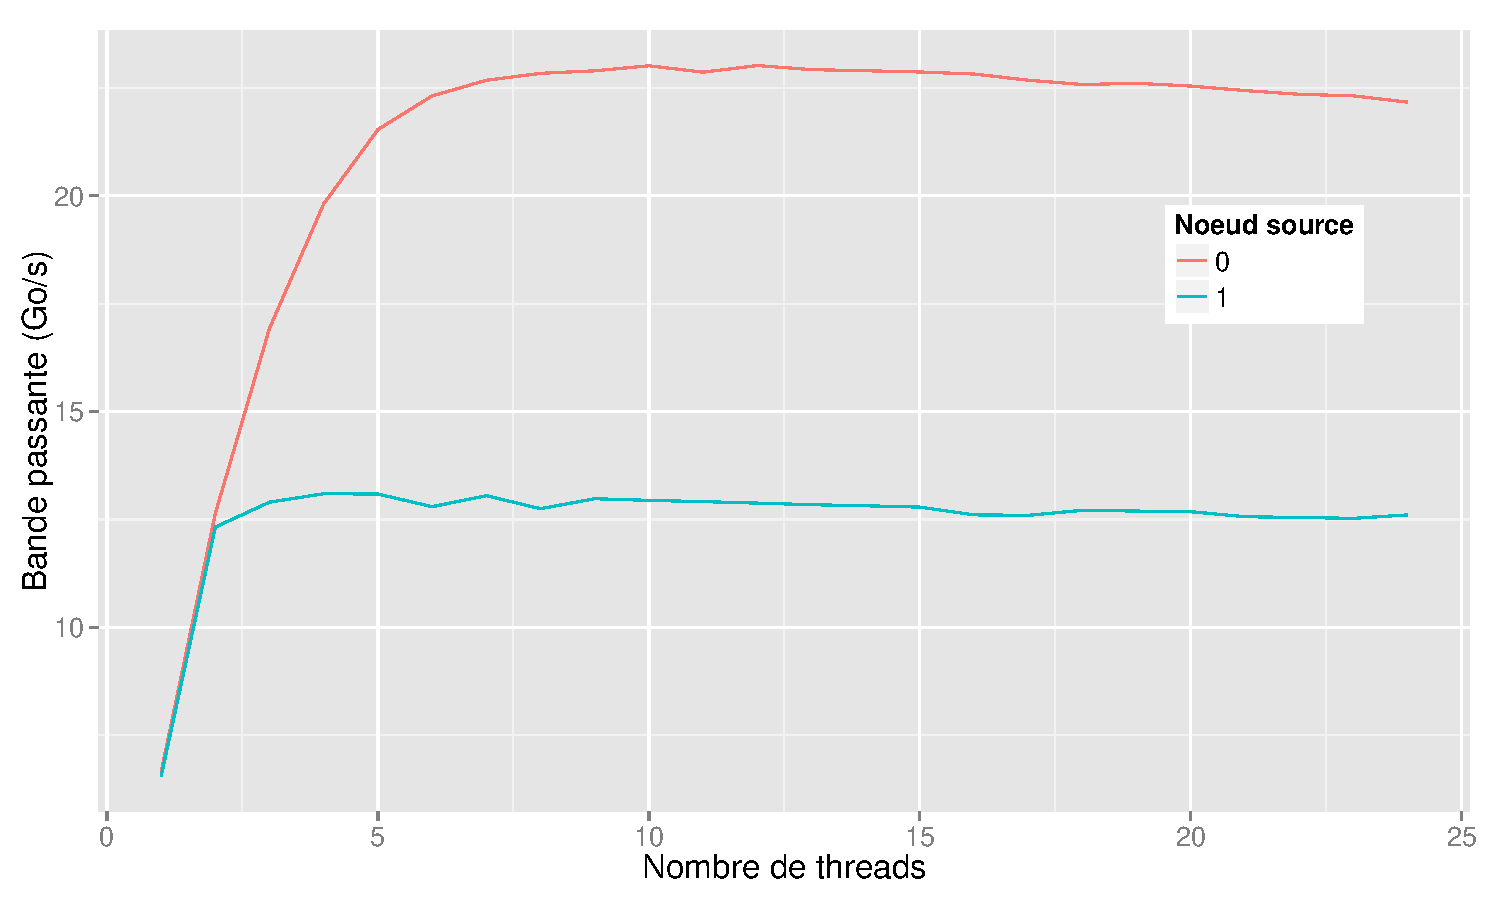
\includegraphics[width=\textwidth]{link_saturation_brunch}
  \caption{Bande passante cumulée vers le nœud 0, en fonction du nombre de threads effectuant une copie et du nœud source}\label{fig:contribs:machines:brunch:saturation}
\end{figure}


La Figure~\ref{fig:contribs:machines:brunch:heatmap} présente la bande passante nœud à nœud en fonction de la source et de la destination, mesurée à l'aide d'une copie de tableau (|memcpy|) de 200 Mo.
Bien qu'une diagonale se dégage clairement, la différence entre accès local et accès distant n'est de l'ordre que de 10\%~: la bande passante point à point pour l'accès local est d'environ 3.6 Go/s, et d'environ 3.3 Go/s pour le point à point sur un nœud distant.

\subsubsection{Mesure des liens}

De même que pour idchire, nous avons effectué des observations complémentaires pour caractériser plus précisément les liens locaux et distants, afin de déterminer leur saturation.
Les résultats de ces expériences ont été rassemblés sur la figure~\ref{fig:contribs:machines:brunch:saturation}.
Il s'agit de la même approche que pour la figure~\ref{fig:contribs:machines:idchire:saturation}, et nous avons effectué des copies simultanées depuis un nœud source vers le nœud 0.

En plus de constater que la bande passante cumulée est bien plus importante que sur idchire, on peut voir que les liens arrivent à saturation avec le même nombre de copies simultanées (environ 6), même si proportionnellement ça ne représente que 20\% d'utilisation du nœud.

\bigskip
\bigskip

Ces résultats sur les capacités physiques des machines vont avoir un impact important dans la section suivante~: nous allons faire une étude de cas d'une application - la factorisation de Cholesky, et nous allons en étudier individuellement les parties critiques.
Certaines de ces parties critiques peuvent utiliser un large ensemble de données, en pleine charge de la machine les performances seront donc limitées par les résultats que nous venons de décrire.

